\documentclass[conference]{IEEEtran}
\IEEEoverridecommandlockouts
% The preceding line is only needed to identify funding in the first footnote. If that is unneeded, please comment it out.
\usepackage{cite}
\usepackage{amsmath,amssymb,amsfonts}
\usepackage{algorithmic}
\usepackage{graphicx}
\usepackage{textcomp}
\usepackage{xcolor}
\usepackage{fancyhdr} % 添加页眉页脚
\usepackage{subfigure}% in preamble
\def\BibTeX{{\rm B\kern-.05em{\sc i\kern-.025em b}\kern-.08em
    T\kern-.1667em\lower.7ex\hbox{E}\kern-.125emX}}
\begin{document}

\title{A Brief Report on Oscillators\\
}

\author{\IEEEauthorblockN{Zhou jy}
\IEEEauthorblockA{\textit{Institute of Media,Information, and Network} \\
\textit{Shanghai Jiao Tong University}\\
Shanghai, China \\
blabla@sjtu.edu.cn}

}

\maketitle
\thispagestyle{fancy} 
\lhead{} % 页眉左,需要东西的话就在{}内添加
\chead{} % 页眉中
\rhead{} % 页眉右
\lfoot{} % 页眉左
\cfoot{\thepage} % 页眉中
\rfoot{} %页眉右,\thepage 表示当前页码
\renewcommand{\headrulewidth}{0pt} %改为0pt即可去掉页眉下面的横线
\renewcommand{\footrulewidth}{0pt} %改为0pt即可去掉页脚上面的横线
\pagestyle{fancy}
\cfoot{\thepage}

\begin{abstract}
This is a report of the course Electronic Circuit ES342-4, the topic of which is oscillator module in RF transceiver system. It will start from the basic concept of oscillators, and briefly introduce the principle, composition, and system model about oscillator. At the same time, it is integrated and summarized based on collected literature and articles, and a brief literature review is conducted from the perspective of important properties of oscillators, specific types of oscillators such as LC oscillator, QVCO, non-sinusoidal oscillators, etc. In addition, simulations and analysis of different types of oscillators have been performed on Multisim. This article is only a general exploration of the content of oscillators, and hopefully it will tighten the foundation in the field of communication-related for further study in the future. 
\end{abstract}

\begin{IEEEkeywords}
oscillators, RF-transceiver, Multisim, simulation
\end{IEEEkeywords}

\section{Introduction of Oscillator}\label{sec1}
Oscillator is an energy conversion device that converts DC energy into AC energy with a certain frequency. It is an electronic component that can be used to generate a repetitive electronic signal (usually a sine wave or a square wave), and the circuit it forms is called an oscillation circuit.

The most basic components of an oscillator are:
\begin{enumerate}
    \item Triode amplifier (acts as an energy control).
    \item positive feedback network (feeds back part of the output signal to the input).
    \item Frequency selection network (selects the desired oscillation frequency, so that the oscillator can oscillate at a single frequency to obtain the desired waveform).
\end{enumerate}


Oscillators can be divided into sine, non-sine oscillators and crystal oscillators, among which sine oscillators mainly include LC oscillators and RC oscillators. RC oscillator uses RC network as the frequency shifting network, and it belongs to the audio oscillator; LC oscillator uses LC oscillation circuit as the positive feedback oscillator of phase shifting and frequency selection network, mainly including the three-point (Hartley) oscillator, Clapp oscillator, Siller oscillator ,etc.The oscillation frequency of crystal oscillator is controlled by quartz crystal, and its main characteristics include very stable physical and chemical properties, positive piezoelectric effect and inverse piezoelectric effect, and the oscillation frequency is the fundamental frequency $\omega_s$.

Oscillator is widely used in electronic industry, medical, scientific research and other aspects, mainly including the major universities, medical, petrochemical, health epidemic prevention, environmental monitoring and other scientific research departments.

In this article, Sec.\ref{sec1} has already described the basic concept and composition of oscillator. Sec.\ref{sec2} will give a brief introduction to the basic principle of oscillator. Sec.\ref{sec3} and Sec.\ref{sec4} will do a literature review of the articles about oscillators, where Sec.\ref{sec3} mainly focuses on the important properties of oscillator, including phase noise, power dissipation, mutual injection pulling, spectrum folding and trade-offs between noise and power; Sec.\ref{sec4} is a brief description of different types of oscillators, including the classification of LC oscillators, quadrature LC CMOS oscillators, and non-sinusoidal oscillators. In addition, Sec.\ref{sec5} also simulates different oscillators through Multisim software, mainly including simple sinusoidal oscillators, crystal oscillator, Siller oscillator, and three-point oscillator. Finally Sec.\ref{sec6} will give a brief summary of the article.

\section{Principle of oscillator}\label{sec2}

The oscillator model has two modules, amplifier and the feedback network, and the signals involved are input signal $V_{in}$, feedback signal $V_f$ and output signal $V_{out}$. We want the oscillator to operate at a certain frequency and need to continuously strengthen the components at that frequency to make them stand out from the thermal noise, which is a process known as "positive feedback". The core of positive feedback is the feedback network, which can be considered as a filter that selects only the frequency component of interest, i.e. the oscillation frequency$\omega_1$. Next, the feedback signal $V_f$, which passes through the feedback network, is in phase with $V_{in}$ at the oscillation frequency, and the two signal are superimposed to become the new $V_{in}$ and then fed into the amplifier for amplification. After each feedback and amplification, the new $V_{in}$ is larger than the previous $V_{in}$ at the oscillation frequency, thus realizing positive feedback.

\begin{figure}[!h]
\centerline{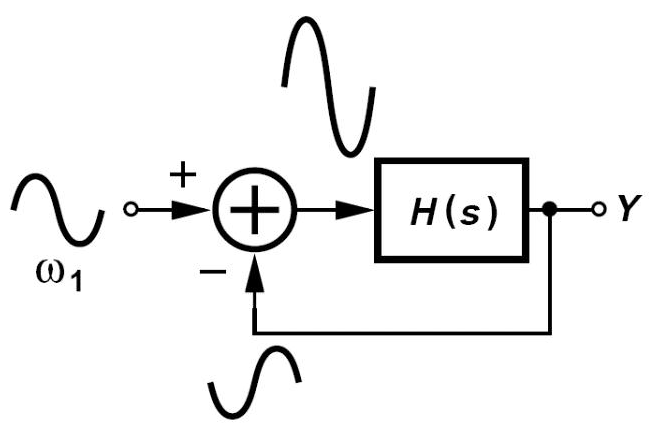
\includegraphics[scale=0.25]{fig/pic2-1.png}}
\caption{Barkhausen's Criteria for oscillators.}
\label{fig2-1}
\end{figure}

For the negative feedback system shown in Fig\ref{fig2-1}, it can only constitute positive feedback if it satisfies Barkhausen's Criteria. When the system transfer function is $H(j\omega_1)=-1$, it will generate a "frequency-dependent" phase shift of 180°, which will constitutes a whole 360 phase shift at frequency $\omega_1$ together with the 180° phase shift of the negative feedback. If the gain of $H(j\omega_1)$ is greater than or equal to 1, the feedback loop will constitute a positive feedback, forming an oscillation at frequency $\omega_1$. Currently, Barkhausen's Criteria is widely used in the design of electronic oscillators.

\section{Important Properties of Oscillator}\label{sec3}
There are many properties related to oscillators, including phase noise, mutual injection pulling, spectrum folding, power dissipation, accuracy, etc. The following several subsections will focus on a number of papers on oscillator-related properties and provide a certain brief description of the relevant content.

\subsection{Phase Noise}\label{Phase Noise}
Phase noise is usually characterized in the frequency domain. For an ideal oscillator operating at $\omega_0$, the spectrum
assumes the shape of an impulse, whereas for an actual
oscillator, the spectrum exhibits “skirts” around the center
or “carrier” frequency (Fig.\ref{fig3-1}). To quantify phase noise, a common method is to consider a unit bandwidth at an offset $\Delta\omega$ with respect to $\omega_0$, calculate the noise power in this bandwidth $\Delta\omega$, and divide the result by the carrier power.

\begin{figure}[!h]
\centerline{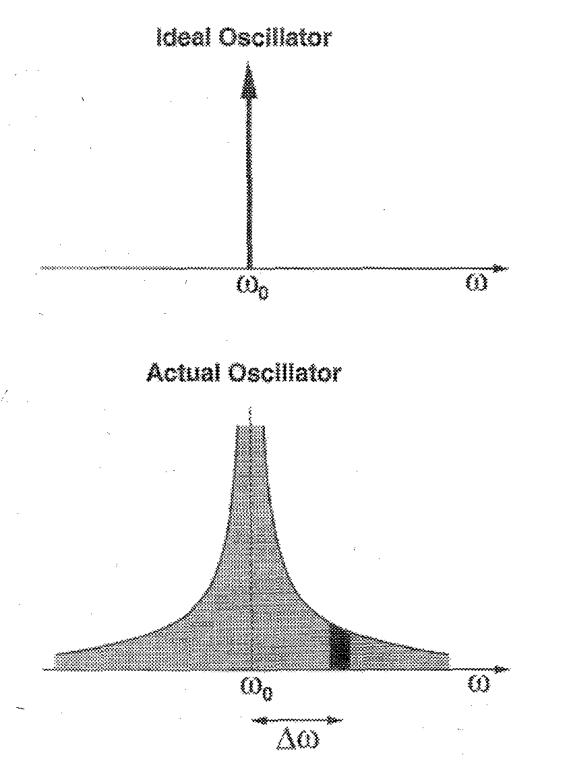
\includegraphics[scale=0.25]{fig/pic3-1.jpg}}
\caption{Phase noise in an oscillator.\cite{b3}}
\label{fig3-1}
\end{figure}

In the paper by B. Razavi\cite{b3}, it presents a study of phase noise in two inductorless CMOS oscillators. They first used a linear model to calculate the CMOS ring oscillators' phase noise. They treat an oscillator as a feedback system and consider each noise source as an input. The system transfer function can be expressed at the resonant frequency $\omega=\omega_0$ as:

\begin{equation}
\frac{Y}{X}(j\omega_0)=\frac{H(j\omega_0)}{1+H(j\omega_0)}
\label{eq3-1}
\end{equation}

For noise component at $\omega = \omega_0 + \Delta\omega$, the noise tranfer function can be shaped as: 
\begin{equation}
|\frac{Y}{X}(j\omega_0+\Delta\omega)|^2=\frac{1}{4Q^2}(\frac{\omega_0}{\Delta\omega})^2
\label{eq3-2}
\end{equation}

where the open-loop Q is defined:
\begin{equation}
Q=\frac{\omega_0}{2}\sqrt{(\frac{dA}{d\omega})^2+(\frac{d\Phi}{d\omega})^2}
\label{eq3-3}
\end{equation}

Therefore, the ring oscillators can be modeled as the linearized model of CMOS VCO shown in Fig\ref{fig3-2}. The noise power spectrum is shaped by:
\begin{equation}
|\frac{V_1}{I_{n1}}(j\omega_0+\Delta\omega)|^2=\frac{R^2}{27}(\frac{\omega_0}{\Delta\omega})^2
\label{eq3-4}
\end{equation}

\begin{figure}[!h]
\centerline{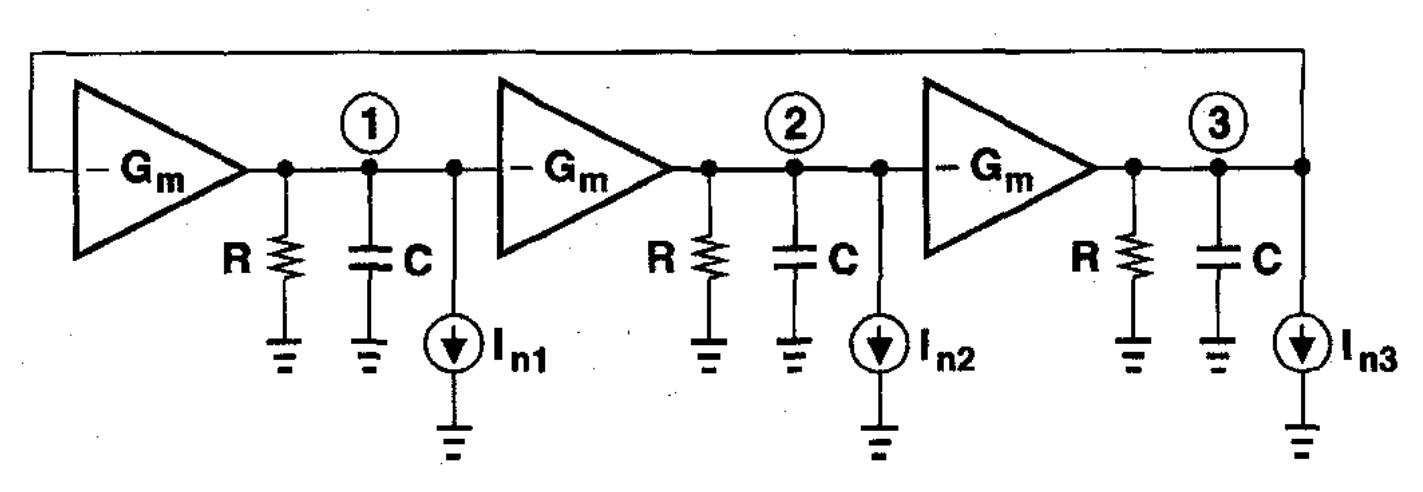
\includegraphics[scale=0.2]{fig/pic3-2.jpg}}
\caption{Linearized model of CMOS VCO.\cite{b3}}
\label{fig3-2}
\end{figure}

Furthermore, nonlinear effects are considered and three phase noise phenomena, namely, additive noise, high-frequency multiplicative noise, and low-frequency multiplicative noise, are identified and formulated. 

Based on the same concepts, a CMOS relaxation oscillator is also
analyzed. For $C_D=0.5C_A$ in Fig.\ref{fig3-4}, Q reaches its maximum value-unity and the timing (floating) capacitor is equal to the load capacitance, thus the noise shaping function is equal to $(\omega_0/\Delta\omega)^2/4$

\begin{figure}[htbp]
	\centering
	\begin{minipage}{0.49\linewidth}
		\centering
		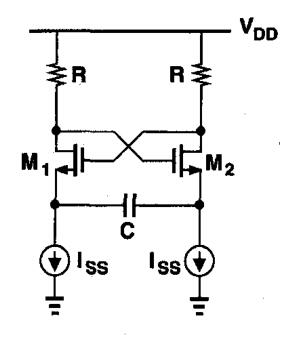
\includegraphics[width=0.7\linewidth]{fig/pic3-3.jpg}
		\caption{CMOS relaxation oscillator}
		\label{fig3-3}%文中引用该图片代号
	\end{minipage}
	%\qquad
	\begin{minipage}{0.49\linewidth}
		\centering
		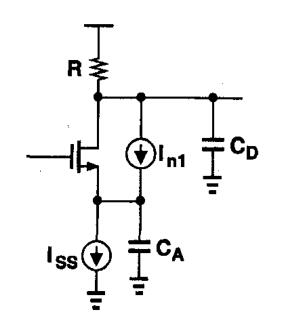
\includegraphics[width=0.7\linewidth]{fig/pic3-4.jpg}
		\caption{Noise calculation}
		\label{fig3-4}%文中引用该图片代号
	\end{minipage}
\end{figure}

\subsection{Mutual Injection Pulling}
The phenomenon of pulling has been studied extensively for a single oscillator under injection of an independent sinusoid in 
Razavi's article\cite{b5}. 

However, in some applications, coupling through the supply and the substrate may lead to mutual pulling between two oscillators. In broadband data transceivers, for example, the transmit PLL and data recovery circuit may operate at slightly different frequencies (because the latter is locked to the incoming data), thus has the probability to pull each other. Furthermore, emerging wireless systems such as ultra wide-band transceivers may incorporate multiple PLLs and must
deal with unwanted mutual pulling.

In paper\cite{b2} of Razavi, it first determines the response of a single oscillator to an independent phase-modulated input. Then, use the pre-calculated conclusions to analyze the mutual injection pulling between two free-running oscillators or PLLs in both time and frequency domains and determine the mathematical expression for the pulled frequency.


\subsection{Spectrum folding}
Samor and his team\cite{b1} assessed the noise performance of a LC Tuned oscillator shown in Fig.\ref{fig3-5} quantitatively by the single sideband-to-carrier ratio (SSCR). They have shown that the nonlinear operation of the transconductor stage has to be properly accounted for since it introduces spectrum folding. Besides, The noise of the tail generator cannot be neglected either and may be dominant if not properly minimized.

The nonlinear behavior of the transconductor causes a folding of the wide-band noise sources like the thermal noise of the transistor spreading resistance. 

\begin{figure}[!h]
\centerline{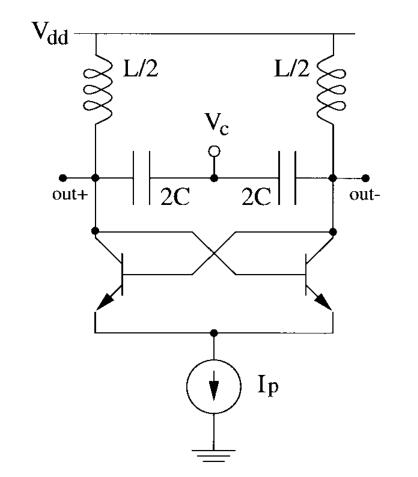
\includegraphics[scale=0.30]{fig/pic3-5.jpg}}
\caption{Schematic structure of a differential LC tuned oscillator.\cite{b1}}
\label{fig3-5}
\end{figure}

In general, the double-sided power spectrum of the output voltage noise at a frequency offset $\alpha$ from the carrier can be written as:
\begin{equation}
S_{nv}(\alpha)=\frac{1}{4}\frac{KT}{C}\frac{\omega_0}{Q}\frac{1}{\alpha^2}(1+F)
\label{eq3-5}
\end{equation}

with a noise factor $F$ given by:
\begin{equation}
F=2r_{bb'} g_{ot} \eta + \frac{\sigma S_{nt}}{KTg_{ot}}
\label{eq3-6}
\end{equation}

Furthermore, it is need to Note that the intermodulations between the carrier and wide-band noise sources cause noise folding that increases the transconductor noise factor $F$.

\subsection{Power Dissipation}
Many works have been reported to improve phase noise which mentioned in section \ref{Phase Noise} and power dissipation based on the conventional topology. It uses additional coupling transistors which performs inherently inferior to the conventional topology in the aspects of phase noise and power dissipation. 

Hye-Ryoung Kim and his team \cite{b4} proposed A new quadrature voltage-controlled oscillator (QVCO) topology which enables quadrature coupling without requiring additional transistors. 

\begin{figure}[!h]
\centerline{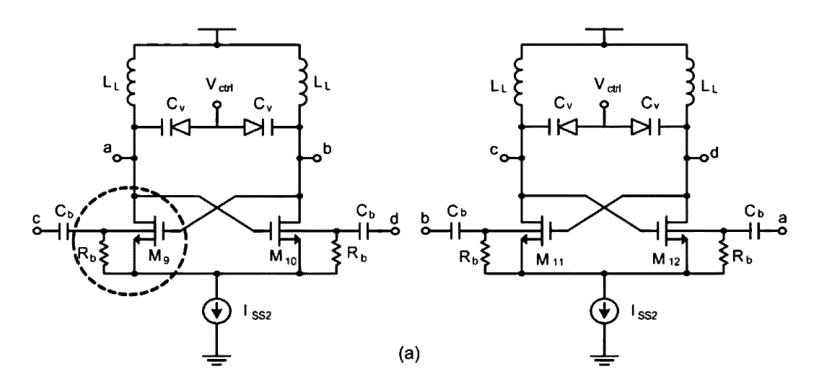
\includegraphics[scale=0.30]{fig/pic3-6.jpg}}
\caption{Back-gate coupled LC-QVCO\cite{b4}}
\label{fig3-6}
\end{figure}

The topology structure is shown in the Fig.\ref{fig3-6}. The quadrature couplings are realized by utilizing the back-gates of the core transistors. The use of back-gates reduces the power dissipation and removes the additional noise contributions compare to the conventional coupling transistor based topology.The advantages of the newly proposed QVCO topology are exploited mainly based on simulation in comparison with prior works.

From the simulation \cite{b4}, the advantages of the proposed QVCO are demonstrated in comparison with the conventional coupled-transistor-based QVCO and the differential VCO. A QVCO based on the proposed topology with additional design ideas has been implemented using a $0.18-\mu m$ triple-well CMOS technology for 1 GHz-band operation. The measurement shows that the phase noise of 120 dBc/Hz at 1-MHz offset with output power of 2.5 dBm, while dissipating only 3 mA for the whole QVCO from 1.8-V supply.

\subsection{Trade-offs between Noise and Power}

In article \cite{b6}, J. Craninckx derived a general notation for the phase noise of LC-tuned oscillators, based on the calculation of transfer functions. Moreover, two important terms were introduced in Eq.\ref{eq3-8}, namely, the effective resistance $R_{eff}$ and the effective capacitance $C_{eff}$. And the distinction between a passive and an active implementation of the inductor is also discussed.

\begin{equation}
\begin{aligned}
C_{eff} &= n\cdot C \\
R_{eff} &= n\cdot R\cdot (\frac{1}{n-1})^2 \approx\frac{R}{n}
\end{aligned}
\label{eq3-8}
\end{equation}

It proposed a LC-tank consisting of n inductors and n capacitors, whose main advantage is to reduce the internal voltage swing while holding the noise constant. This should limit the coupling between the oscillator and other circuits integrated on the same die. This leads to the following expressions about the phase noise and power consumption for passive inductors:

\begin{equation}
\begin{aligned}
dV_{out}^2\{\Delta \omega\} &= \frac{2KT}{n\omega_0C}\cdot N\cdot (\frac{\omega_0}{\Delta\omega})^2\cdot df \\
G_M &= 2n\cdot \omega_0 C
\end{aligned}
\label{eq3-7}
\end{equation}

The formula for active inductors is basically the same and will not be repeated here. Eq.\ref{eq3-7} shows the perfect trade-off that can be made: phase noise decreases proportionally with n, power and area increase proportionally with n. 

Using the concepts derived in this paper \cite{b6}, several kinds of LC-tanks can be developed and analyzed, resulting in an optimum solution for cellular-telephone applications.

\section{Brief description of specific oscillators}\label{sec4}
This section will mainly focus on specific oscillators, including a discussion of the classification of LC oscillators and a detailed introduction to CMOS LC quadrature VCOs, with some collection and integration of related literature.

\subsection{Classification of LC Oscillators}

A systematic synthesis procedure is given for classifying a class of LC oscillators \cite{b7}. According to previous description in Sec \ref{Introduction}, an oscillator shown in Fig.\ref{fig4-1} basically consists of an amplifier and a passive network N in its feedback path.

When gain A of the amplifier is negative real, one additional buffer amplifier is possibly required. It is shown that if OA-based amplifier is used for realizing A, the synthesized oscillators is not influenced by the input and output impedances of the OA. Thus, Rathore build an oscillator model with the most general 2-port passive network N and an OA-based amplifier \cite{b7}. Since a 2-port passive network N can be represented by either $\pi$ or $T$ network, it will get all 12 possible oscillators. 

\begin{figure}[!h]
\centerline{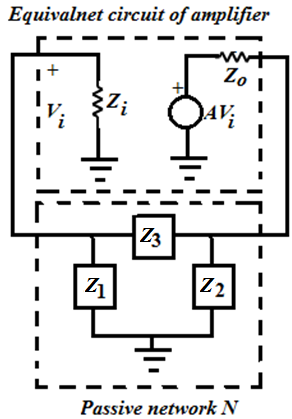
\includegraphics[scale=0.5]{fig/pic4-1.png}}
\caption{Basic oscillator circuit with equivalent circuit
of amplifier and passive network N as $\pi$ network \cite{b7}}
\label{fig4-1}
\end{figure}

For the $\pi$-network shown in Fig.\ref{fig4-1}, twelve types of oscillators can be formed by changing the types of Z1 and Z2. For example, $Z_1$ and $Z_2$ can be designed of similar nature or opposite nature, and they can both choose between capacitance or inductance. As a result, the passive network can be classified as $\pi$-network into 6 categories. Besides, it is interesting to note that the top 2 $\pi$-networks shown in Fig.\ref{fig4-2} can be converted to the two which located in the center left and center bottom of the Fig.\ref{fig4-2} respectively by interchanging input and ground. Meanwhile, it is also shown that the set of 6 oscillators when N is a $\pi$-type network can be easily converted into another set of 6 oscillators when N is a T-type as shown in Fig.\ref{fig4-3}. 

\begin{figure}[!h]
	\centering
	\begin{minipage}{0.49\linewidth}
		\centering
		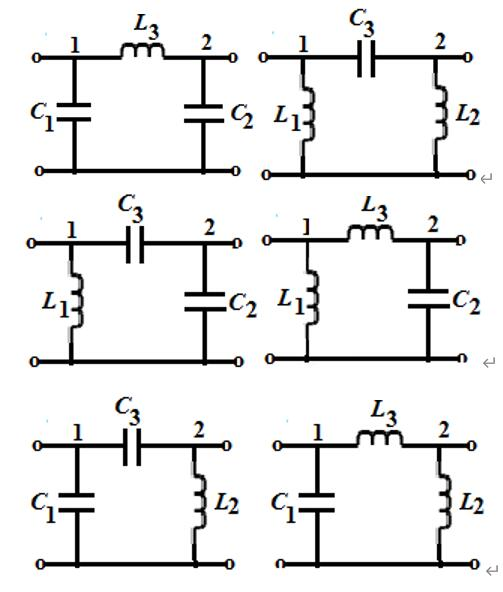
\includegraphics[width=0.7\linewidth]{fig/pic4-2.jpg}
		\caption{$\pi$-network}
		\label{fig4-2}%文中引用该图片代号
	\end{minipage}
	%\qquad
	\begin{minipage}{0.49\linewidth}
		\centering
		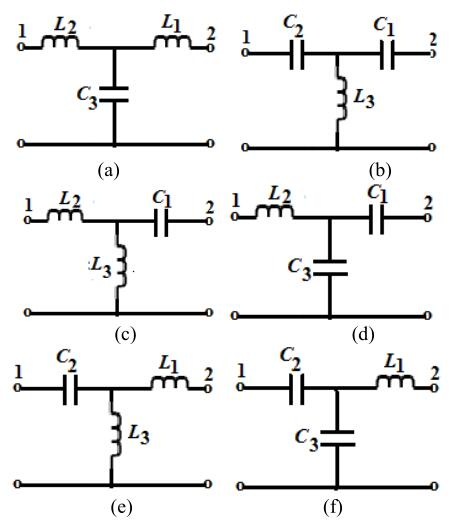
\includegraphics[width=0.7\linewidth]{fig/pic4-3.jpg}
		\caption{T-network}
		\label{fig4-3}%文中引用该图片代号
	\end{minipage}
\end{figure}

It can be concluded that all the 12 oscillators have been classified into various groups based on various factors. And some of the oscillators can be converted into some others by complimentary transformation.

\subsection{CMOS LC Quadrature VCO}
Local oscillators with quadrature outputs (referred to as quadrature oscillators, QOs) are key building blocks in many wireless and wired communication systems. 

The literature \cite{b8} presented an analytic approach for the estimation of the phase and amplitude imbalances caused by component mismatches and parasitic magnetic fields in two popular quadrature LC oscillators. 
\begin{figure}[!h]
\centerline{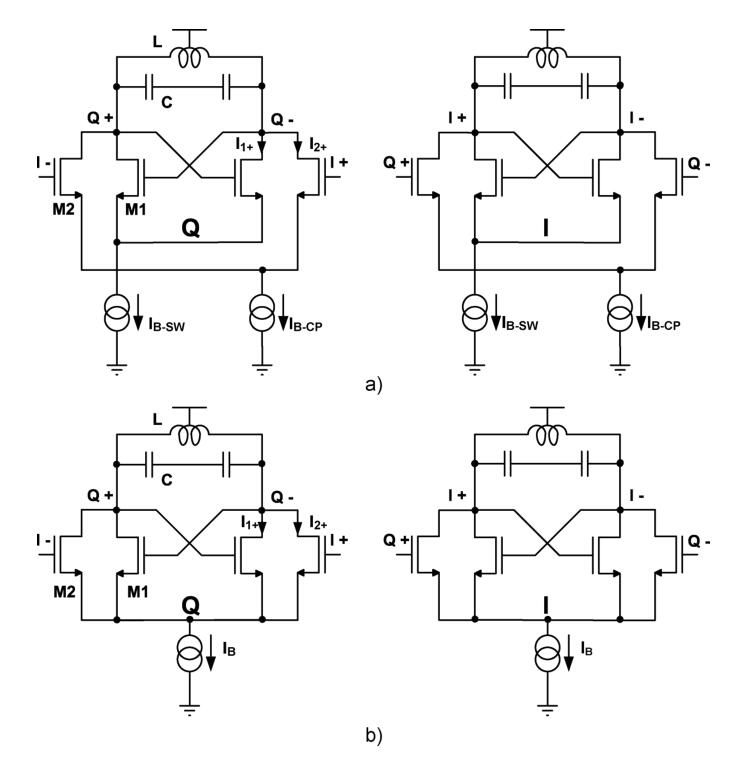
\includegraphics[scale=0.35]{fig/pic4-4.jpg}}
\caption{Circuit schematic of (a) disconnected-sources (DS) QO and (b) connected-sources (CS) QO.\cite{b8}}
\label{fig4-4}
\end{figure}

The two popular parallel-coupled QOs are showed in Fig.\ref{fig4-4}. Two identical oscillators, I and Q, are connected to each other by means of two additional differential pairs. While in Fig.\ref{fig4-4}-a, the direct connection from Q to I and cross-connection of I to Q ensures a quadrature relation between the phases of the output waveforms, which is called a disconnected-sources (DS) QO. The other QOs in Fig.\ref{fig4-4}-b  shows a slightly different implementation, it is derived from DSQO simply by connecting together the common source nodes of the differential pairs driving the I-tank and the Q-tank.Besides, the bias currents $I_{B-CP}$ and $I_{B-SW}$ are merged together and replaced by a single current source $I_B$. As a consequence, the structure in Fig.\ref{fig4-4}-b is called a connected-sources (CS) QO. 

Although the two quadrature oscillators are deceptively similar, and in fact also share the same small-signal equivalent circuit, their behavior in presence of the two mentioned causes of waveform imbalances is very distinct: the DS-QO is much more sensitive to mismatches than the CS-QO, while the opposite is true if a parasitic magnetic coupling between the oscillator inductors is present. In particular, while in the circuit of Fig.\ref{fig4-4}-a, both inductive coupling and components mismatch limit the achievable phase accuracy between I and Q waveforms. While the CSQO in Fig.\ref{fig4-4}-b is much less sensitive to components mismatch and the achievable accuracy is ultimately limited by inductive coupling. 

As for theoretical analysis, the amplitude and phase errors can be written in the following mathematical expression \cite{b8}:
\begin{equation}
\begin{aligned}
DS-QO &: 
\begin{cases}
\epsilon\approx\frac{Q}{m}(\frac{\Delta L}{L}+\frac{\Delta C}{L}) \\
\phi_e\approx-\frac{1}{2m}\frac{\Delta R}{R}+\frac{1}{2}\frac{Q}{m^2}(\frac{\Delta L}{L}+\frac{\Delta C}{L})
\end{cases}\\
CS-QO &: 
\begin{cases}
\epsilon\approx\frac{1}{2}\frac{\Delta R}{R}+\frac{Q}{2}(\frac{\Delta L}{L}+\frac{\Delta C}{L}) \\
\phi_e\approx-\frac{\Delta R}{R}
\end{cases}
\end{aligned}
\label{eq4-1}
\end{equation}

From the Eq.\ref{eq4-1}, it can conclude that the CS-QO generates much more ideal quadrature waveforms than the DS-QO for the same amount of mismatch between ideally identical components, since the phase error in the CS-QO is insensitive to mismatches between the reactors in the resonators, while the phase error in the DS-QO depends strongly on them. On the other hand, while it is true that amplitude imbalances affect the CS-QO much more than the DS-QO, we have seen that such imbalances are usually much less detrimental than phase errors.

Mazzanti also presents a time-variant analysis of the $1/f$ MOS device noise upconversion into $1/f^3$ phase noise for DSQO and CSQO in another article \cite{b9}. Based on the developed analysis, it also presented that DS-QO is probably the best choice if the phase noise should be kept to a minimum. However, when the close-in phase noise is of a lesser concern, the CS-QO displays a better far-out phase noise than the DS-QO, for the same current consumption, and a lower sensitivity of the quadrature accuracy to component mismatches.

The DS-QO and CS-QO discussed above both belong to Parallel LC-Tank Quadrature Oscillators, as the best known realization of QVCOs, which often referred to as the P-QVCO. However, the paper \cite{b10} presented a new design for a quadrature CMOS VCO, which is called a S-QVCO, it relies on the well-known technique of locking two independent LC VCOs to each other, but where the transistors coupling the two VCOs are placed in series with the cross-coupled switches implementing the negative resistances, rather then in parallel. 

Andreani developed a simplified linear model for both S-QVCO and P-QVCO, and the model has been used to derive the oscillation frequency of the QVCOs, and the influence of the various $1/f$ noise sources on the generation of phase noise in the $1/f^3$ region.The phase-noise figure-of-merit (FoM) for the S-QVCO is calculated according to the commonly
adopted expression:
\begin{equation}
FoM=10log((\frac{f_c}{\Delta f})^2\frac{1}{L(\Delta f)P})
\label{eq4-2}
\end{equation}

where $f_c$ is the oscillation frequency, $\Delta f$ is the offset frequency, and $P$ is the power consumption in milliwatts. The simulated noise difference between P-QVCO and S-QVCO is approximately 9 dB. This analysis provides quantitative results which agree well with the outcome of phase noise simulations performed with SpectreRF, indicating that the S-QVCO has superior performances when compared to the P-QVCO.

\subsection{Non-sinusoidal Oscillator}
As is mentioned in CHAO ZHOU's article \cite{b11}, continuous casting mold is regarded as the heart of the caster, in which non-sinusoidal oscillator is regarded as one of the key technologies to realize highly efficient continuous casting. In casting industry, non-sinusoidal oscillation has the advantages of shorter negative strip time, longer positive strip time, larger negative strip distance, etc. 

Currently, non-sinusoidal oscillation research mainly focuses on the oscillation waveform function and oscillator. Therefore, the non-sinusoidal oscillator with lower cost, high reliability and precision is pursued by metallurgical industry. 

In CHAO ZHOU's paper, a non-sinusoidal oscillator driven by double servomotors was proposed which oscillation waveform and modification ratio can be adjusted during the operation \cite{b11}. And the amplitude can be changed with the oscillator stopping. Since the servomotor rotates in a single direction continuously,  the angular speed $\omega$ of the servomotor can be expressed as:
\begin{equation}
\omega=|\frac{2M\pi fi[1+tan^2(\pi ft)]}{1+[Mtan(\pi ft)]^2}|
\label{eq4-3}
\end{equation}

For the non-sinusoidal oscillator, its oscillation waveform can be expressed in terms of the displacement function, velocity function and the acceleration function. Different waveforms depend on different modification ratios $\alpha$, which is shown in Fig.\ref{fig4-5/6/7/8}.

\begin{figure}[!h]
\centering
\subfigure[Displacement curves.]{
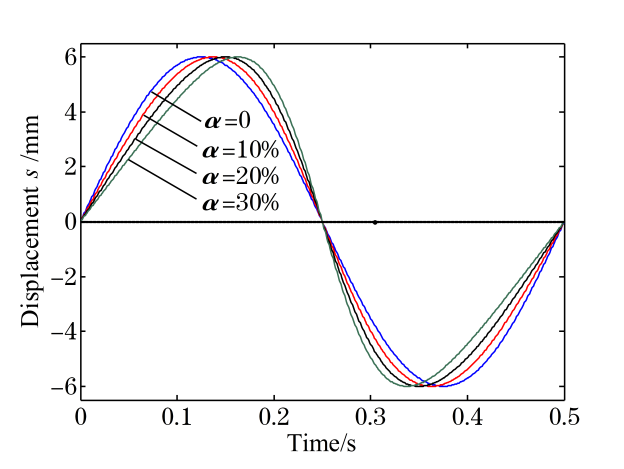
\includegraphics[width=3.9cm]{fig/pic4-5.png}
%\caption{fig1}
}
\quad
\subfigure[Velocity curves.]{
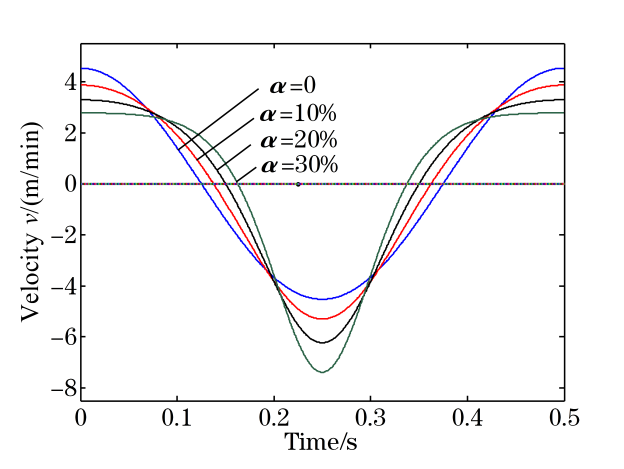
\includegraphics[width=3.9cm]{fig/pic4-6.png}
%\caption{fig1}
}
\quad
\subfigure[Acceleration curves.]{
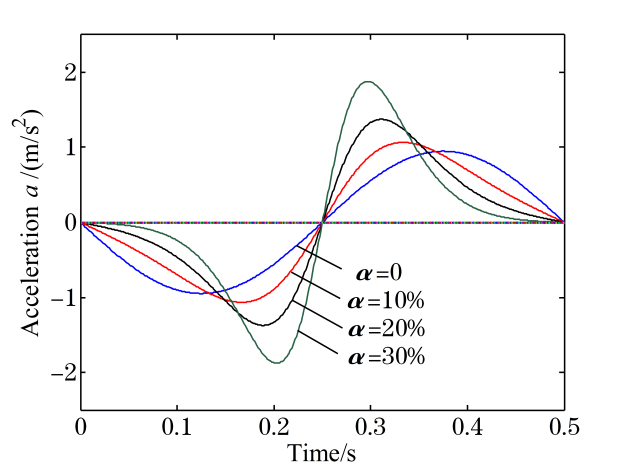
\includegraphics[width=3.9cm]{fig/pic4-7.png}
%\caption{fig1}
}
\quad
\subfigure[ Angular speed.]{
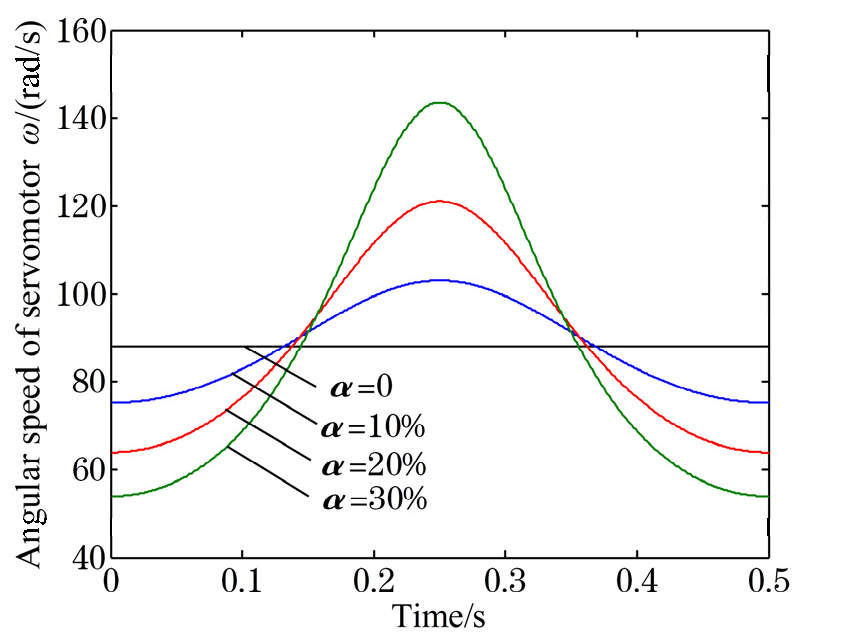
\includegraphics[width=3.9cm]{fig/pic4-8.png}
}
\caption{Non-sinusoidal oscillation waveform with different modification ratios $\alpha$.}
\label{fig4-5/6/7/8}
\end{figure}

For the oscillator, by controlling the angular speed of double servomotors, all the oscillation waveform can be realized, and the sinusoidal and non-sinusoidal waveform can be switched on line conveniently. 

In order to verify the correctness of the oscillation waveform,  a experiment prototype was designed and manufactured in the article \cite{b11}. By comparing the theoretical and tested velocity curves, it can be seen that the theoretical and tested curves are in good agreement. The non-sinusoidal oscillation waveform can be realized accurately with the change of the angular speed of the servomotor rotation and the errors of velocity and displacement waveform are very small. It really provide important guide about the design of non-sinusoidal oscillator for further study and application in oscillation industry. 

\section{Simulation Experiments}\label{sec5}
In the simulation experiments, data collection and simulation implementation of the simulation experiments about Oscillator were carried out, mainly using Multisim software. This includes experiments involved in the analog electricity course like the RC sine oscillator and the Wen’s bridge sine wave oscillator, as well as the simulation of the crystal oscillator, the three-point oscillator, and the Siller oscillator.

In the following subsections, the simulation experiments and results will be briefly described and analyzed in turn. 

\subsection{Simple Sinusoidal Oscillator}
Firstly, for the RC sine wave oscillator, which has been covered in the analog electronics course, the designed simulation circuit is shown in Fig.\ref{fig5-1}. 
\begin{figure}[!h]
\centerline{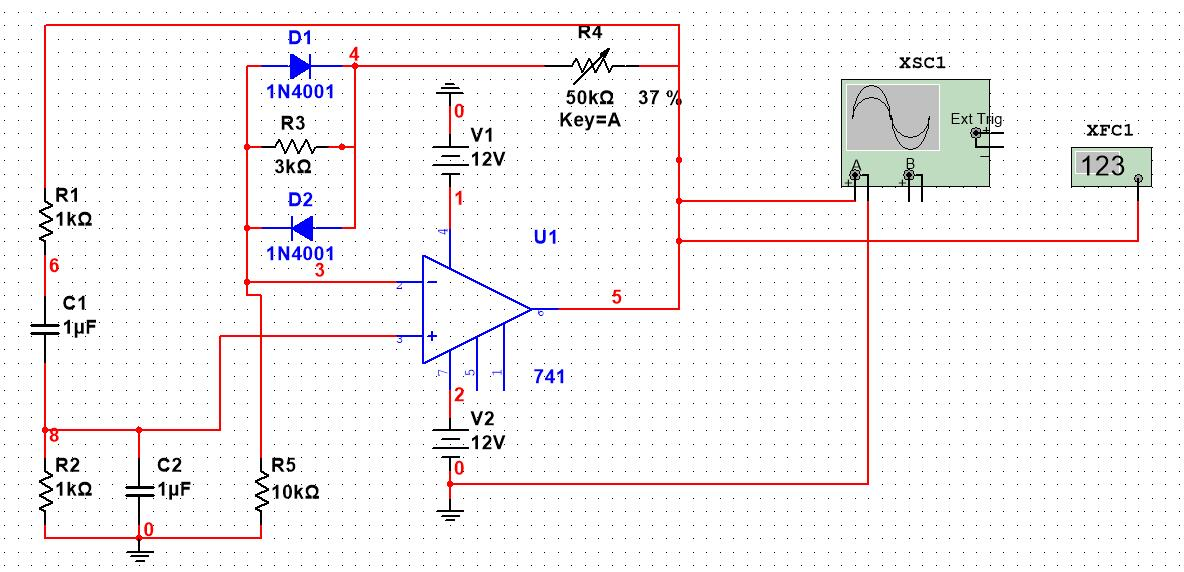
\includegraphics[scale=0.2]{fig/pic5-1.jpg}}
\caption{Simulation of RC sine wave oscillator}
\label{fig5-1}
\end{figure}

Fig.\ref{fig5-2/3} and Fig.\ref{fig5-2/3} respectively shows the simulation results of the initial and stable oscillation stage. After simulation, the oscillation period of the simulation circuit can be derived from the oscilloscope for about 6.25ms, thus the oscillation frequency is $f_0=\frac{1}{6.25ms}\approx 160Hz$. Meanwhile, according to theoretical calculations, we can obtain $f_0=\frac{1}{2\pi\sqrt{R_1R_2C_1C_2}}\approx159Hz$, which is basically consistent to the simulation results. 

\begin{figure}[!h]
\centering
\subfigure[Early stage of vibration.]{
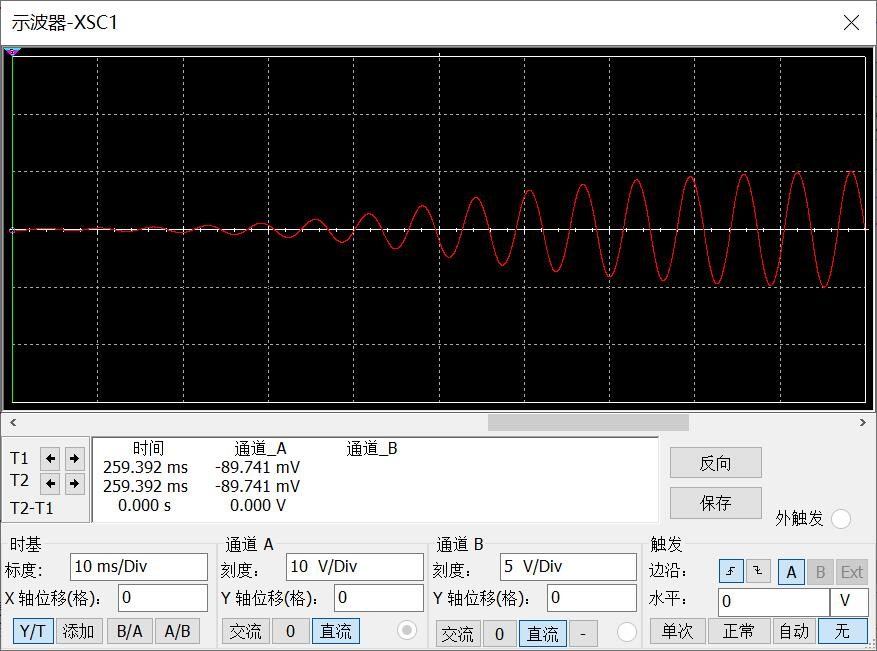
\includegraphics[width=6cm]{fig/pic5-2.jpg}
%\caption{fig1}
}
\quad
\subfigure[Stable oscillation state.]{
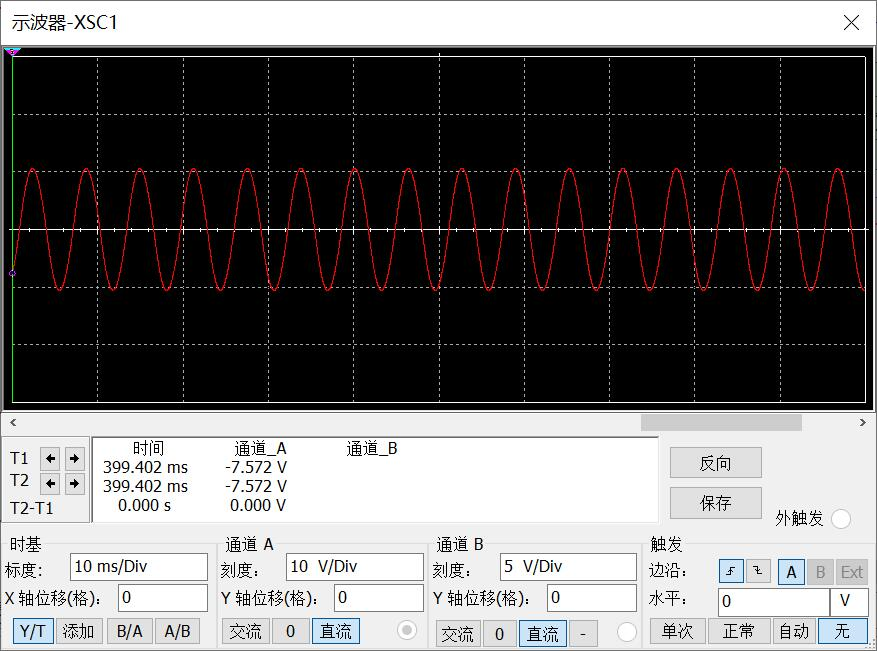
\includegraphics[width=6cm]{fig/pic5-3.jpg}
}
\caption{Simulation results of RC sine wave oscillator}
\label{fig5-2/3}
\end{figure}

The oscillation period depends on $R_1, R_2, C_1, C_2$, the start time of the oscillation depends on $R_3$, and the waveform depends on $R_4$.  The key A ($R_4$) could change the depth of the negative feedback, allowing the circuit to produce several different output signals for stable oscillation, deactivation, and waveform distortion.


\begin{figure}[!h]
\centering
\subfigure[Results after decreasing $R_4$.]{
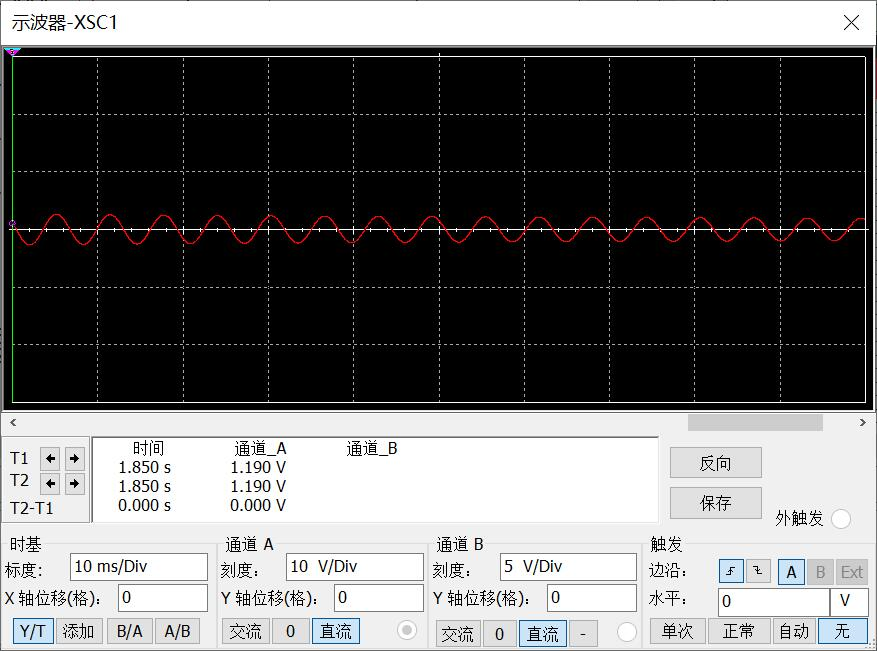
\includegraphics[width=6cm]{fig/pic5-4.jpg}
%\caption{fig1}
}
\quad
\subfigure[Results after increasing $R_4$.]{
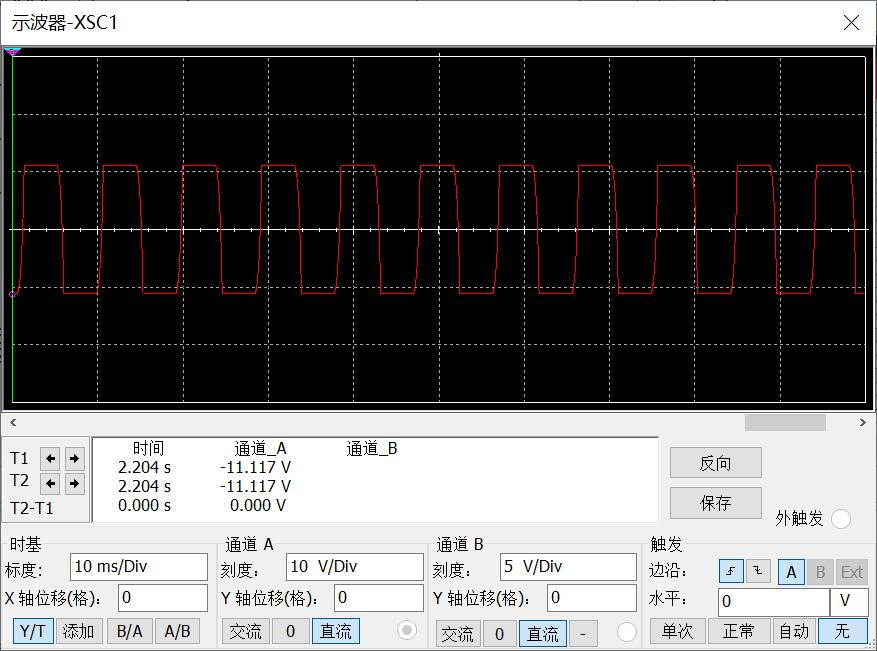
\includegraphics[width=6cm]{fig/pic5-5.jpg}
}
\caption{Experiments about changing $R_4$}
\label{fig5-4/5}
\end{figure}

If we reduce $R_4$ from $18.5K$ to $17K$, we can find that the overall amplitude decreases significantly from the Fig.\ref{fig5-4/5}, and if we continue to reduce $R_4$, the oscillation will stop generating; if we increase $R_4$, the overall amplitude of the oscillation waveform becomes significantly larger and distortion appears at the top of the waveform, and when $R_4=50K$, the oscillation waveform basically approximates a square wave as shown in Fig.\ref{fig5-4/5}. 

\begin{figure}[!h]
\centerline{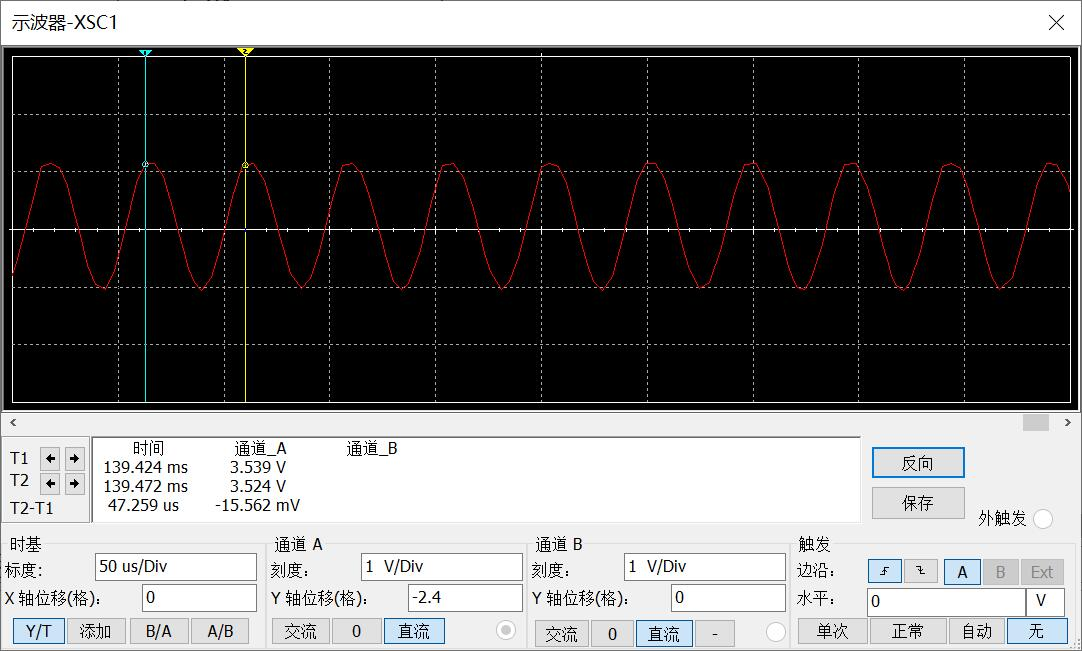
\includegraphics[scale=0.25]{fig/pic5-6.jpg}}
\caption{Simulation of Single-supply Wen's bridge sine wave oscillator}
\label{fig5-6}
\end{figure}

In addition, I also conducted a simulation experiment on a single-supply Wen's bridge sine wave oscillator, and the results are shown in Fig.\ref{fig5-6}. The frequency of the generated sine wave can be determined by an oscilloscope or frequency counter to be about $21.15kHz$. 

\subsection{Crystal Oscillators}
The schematic diagrams of the series and parallel crystal oscillator circuits are shown in Fig.\ref{fig5-7} and \ref{fig5-8}. 

In the series crystal oscillator, the crystal is connected between two points where the oscillator requires low impedance, and is usually connected in the feedback circuit as shown in Fig.\ref{fig5-7}. When the resonant frequency of the circuit is equal to the series resonant frequency of the crystal, the impedance of the crystal is the smallest and approximates a short route, and the circuit can be regarded as an oscillator with capacitive feedback; for the c-b type parallel crystal oscillator, the crystal is connected between the collector and the base, and it is similar to a Clapp oscillator. Since the $C_q$ is very small, the coupling capacitance between the resonant circuit of the crystal oscillator and the oscillation tube is very weak, which makes the frequency stability much higher and the circuit can easily meet the starting conditions. 

\begin{figure}[!h]
	\centering
	\begin{minipage}{0.49\linewidth}
		\centering
		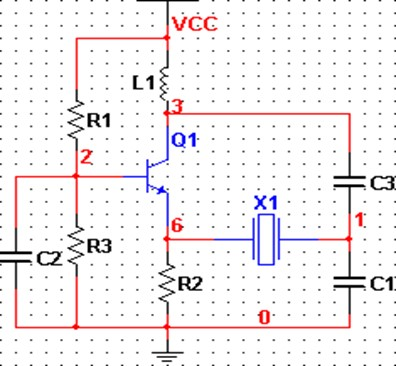
\includegraphics[width=0.72\linewidth]{fig/pic5-7.jpg}
		\caption{Series crystal oscillator.}
		\label{fig5-7}%文中引用该图片代号
	\end{minipage}
	%\qquad
	\begin{minipage}{0.49\linewidth}
		\centering
		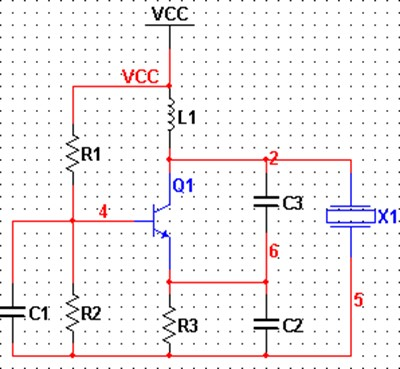
\includegraphics[width=0.72\linewidth]{fig/pic5-8.jpg}
		\caption{Parallel crystal oscillator.}
		\label{fig5-8}%文中引用该图片代号
	\end{minipage}
\end{figure}

Simulation circuits for series and parallel crystal oscillators were designed on Multisim as shown in Fig.\ref{fig5-9/10}. For the series-type transistor oscillator, it can be found that the oscillation waveform is not a single frequency sine wave as shown in Fig.\ref{fig5-12}, but consists of multiple frequency components, and the overall oscillation waveform has a frequency of $2.54MHz$; while for the parallel-type crystal oscillator, its output is approximately a sine waveform from the oscilloscope waveform, and the main frequency component in the spectrum diagram is at $12.67 MHz$ as shown in Fig.\ref{fig5-13/14}, which is approximately the same as the frequency calculated in the oscilloscope and frequency counter, so it can be inferred that the parallel-type crystal oscillator has a better frequency stability.

\begin{figure}[!h]
\centering
\subfigure[Simulation of Series crystal oscillator.]{
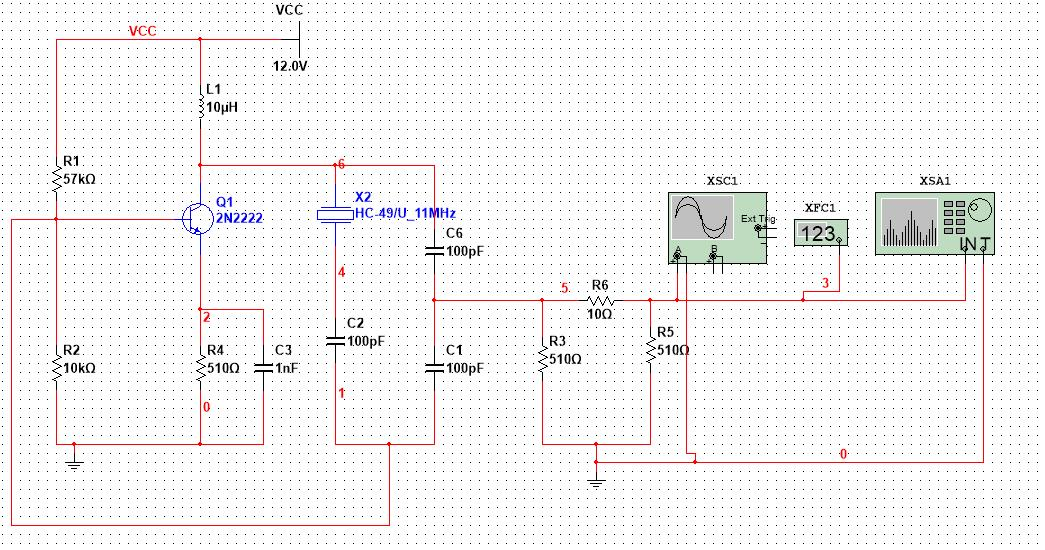
\includegraphics[width=7cm]{fig/pic5-9.jpg}
%\caption{fig1}
}
\quad
\subfigure[Simulation of Parallel crystal oscillator.]{
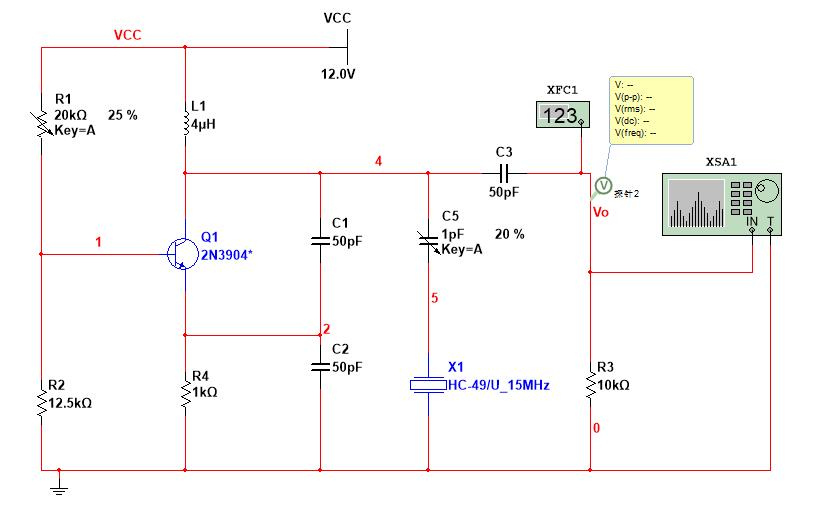
\includegraphics[width=5.7cm]{fig/pic5-10.jpg}
}
\caption{Simulation Circuits of Crystal Oscillators}
\label{fig5-9/10}
\end{figure}


\begin{figure}[!h]
\centerline{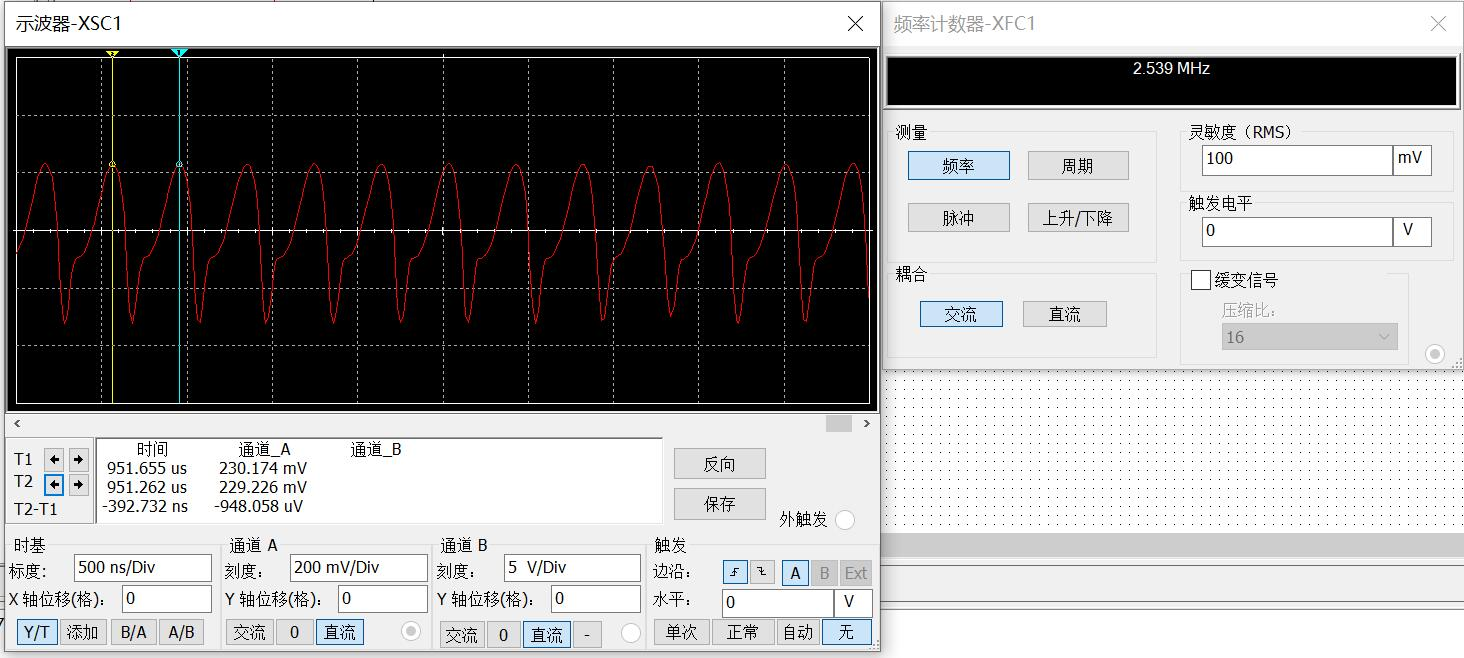
\includegraphics[scale=0.2]{fig/pic5-12.jpg}}
\caption{Simulation results of Series Crystal Oscillators.}
\label{fig5-12}
\end{figure}

\begin{figure}[!h]
\centering
\subfigure[Waveform Graph.]{
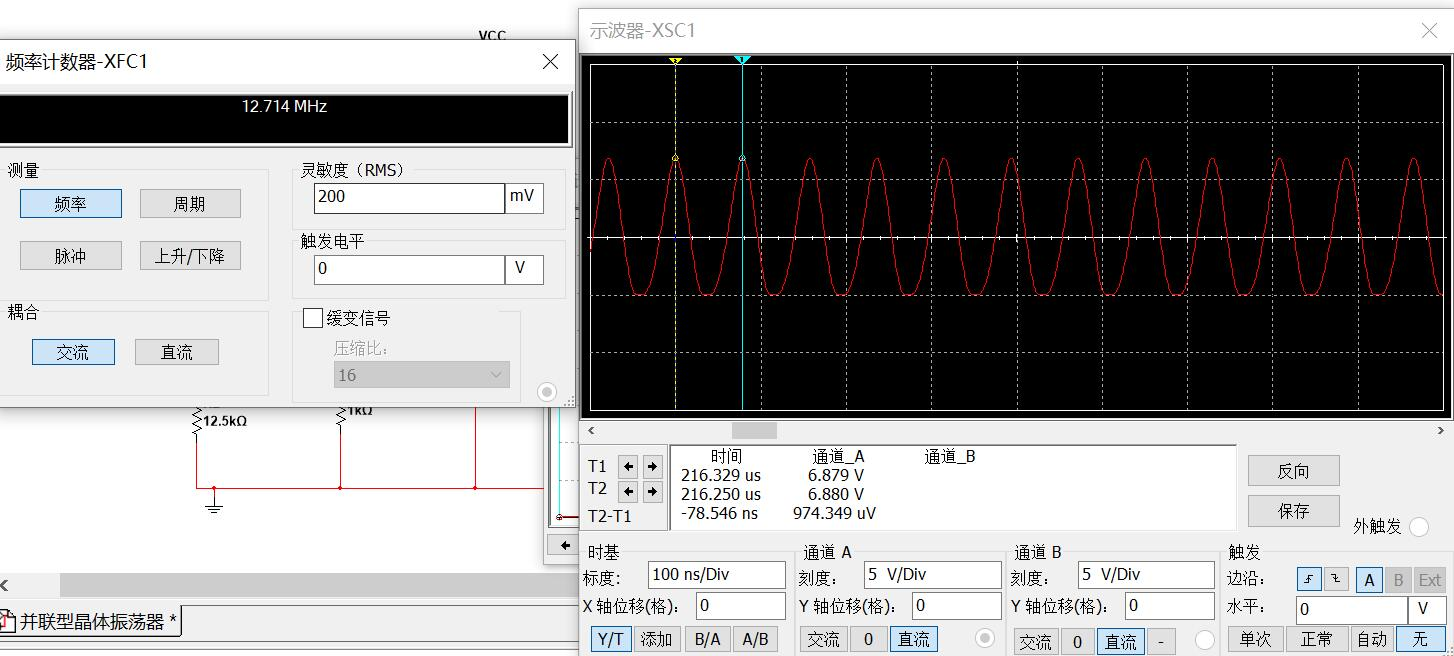
\includegraphics[width=3.9cm]{fig/pic5-13.jpg}
%\caption{fig1}
}
\quad
\subfigure[spectrum diagram.]{
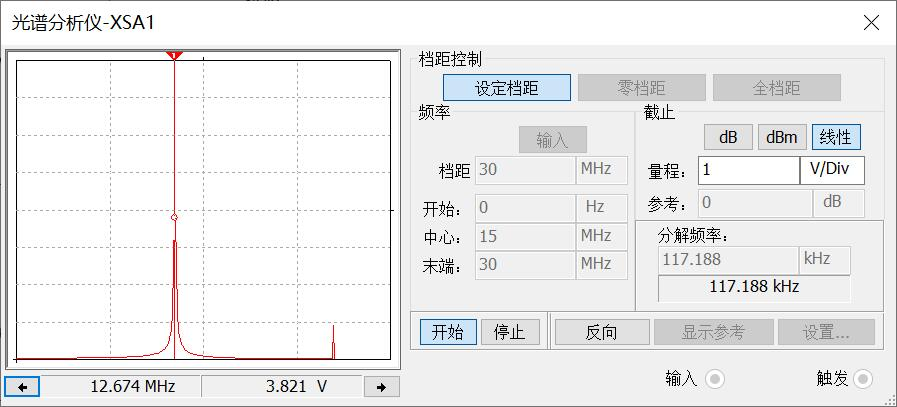
\includegraphics[width=3.9cm]{fig/pic5-14.jpg}
}
\caption{Simulation results of Parallel Crystal Oscillators.}
\label{fig5-13/14}
\end{figure}

\subsection{Siller Oscillator}
The system circuit principle structure of the Siller oscillator is shown in Fig.\ref{fig5-15}. Siller oscillator is based on the Clapp oscillator. Its circuit is characterized by a capacitor $C_4$ and connected in parallel to both ends of the inductor L. The effect is to maintain the weak coupling between the transistor and the oscillation circuit, making the oscillation frequency stable and adjustable in a wide range. 

\begin{figure}[!h]
\centerline{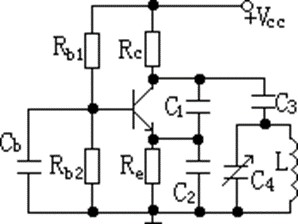
\includegraphics[scale=0.6]{fig/pic5-15.jpg}}
\caption{The schematics diagram of Siller Oscillator.}
\label{fig5-15}
\end{figure}

According to theoretical calculations, the oscillation frequency of the Siller oscillation circuit is obtained as:
\begin{equation}
f_0=\frac{1}{2\pi \sqrt{L(C_3+C_4)}}
\label{eq5-1}
\end{equation}

According to the schematics diagram, circuit diagram is completed in Multisim software environment as shown in Fig.\ref{fig5-16}.
\begin{figure}[!h]
\centerline{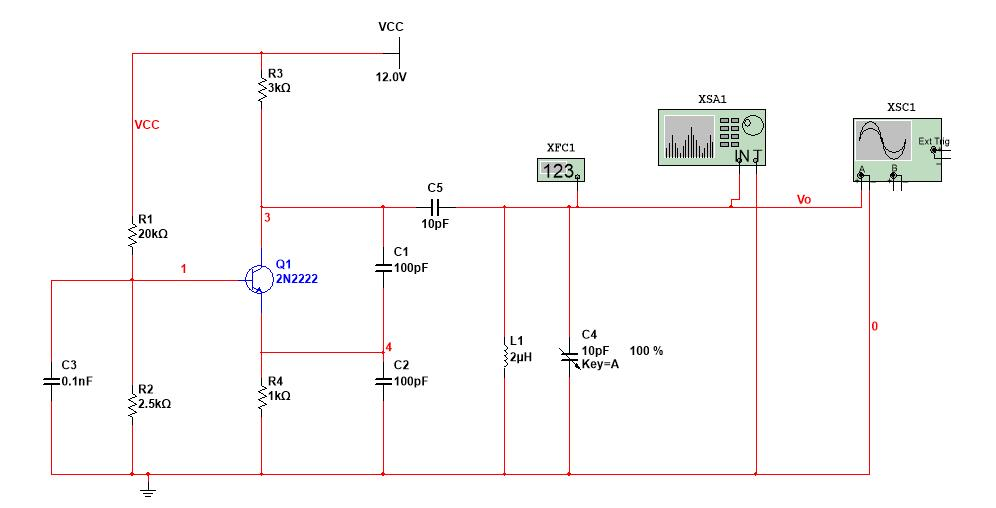
\includegraphics[scale=0.3]{fig/pic5-16.jpg}}
\caption{Simulation circuit of Siller oscillator.}
\label{fig5-16}
\end{figure}

According to result of the frequency counter and the Spectrum Analyzer as shown in Fig.\ref{fig5-17}, the current oscillation circuit frequency is about $26.15MHz$, and the output waveform is an approximate single frequency sine signal, which is close to the theoretical calculation result. 
\begin{figure}[!h]
\centerline{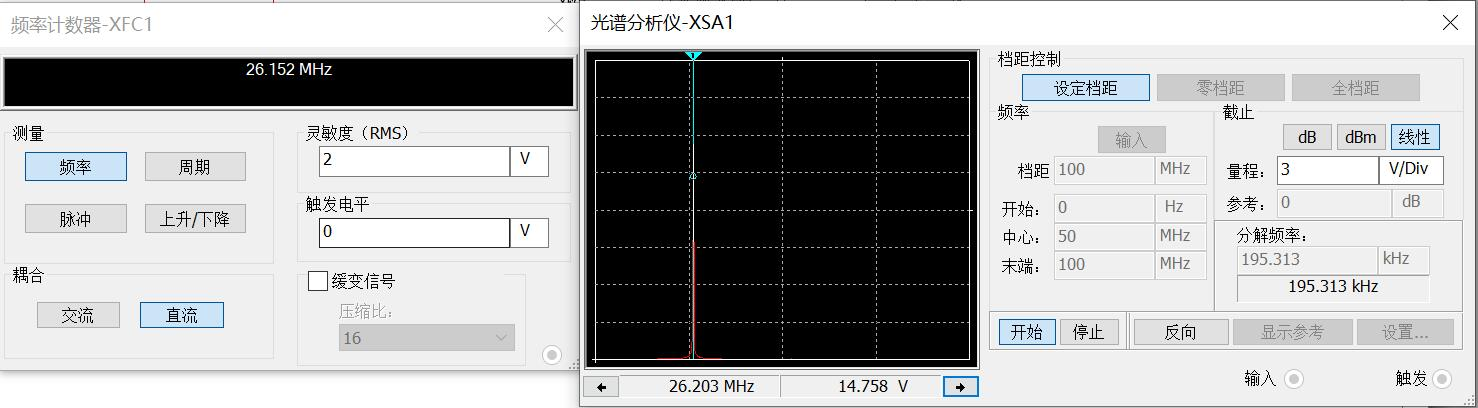
\includegraphics[scale=0.2]{fig/pic5-17.jpg}}
\caption{Simulation results of Siller oscillator.}
\label{fig5-17}
\end{figure}

Next, I performed a simulation analysis in the time domain, executed Simulate Analyses to select transient analysis, set the start time of the simulation to zero, set the end time of the simulation to 5 microseconds, and set the output signal $V_o$ of the simulation as the target of observation. After executing the simulation program, the waveform of the output signal could be seen as shown in Fig.\ref{fig5-18/19/20} -a. 

\begin{figure}[!h]
\centering
\subfigure[Results of the original circuit diagram.]{
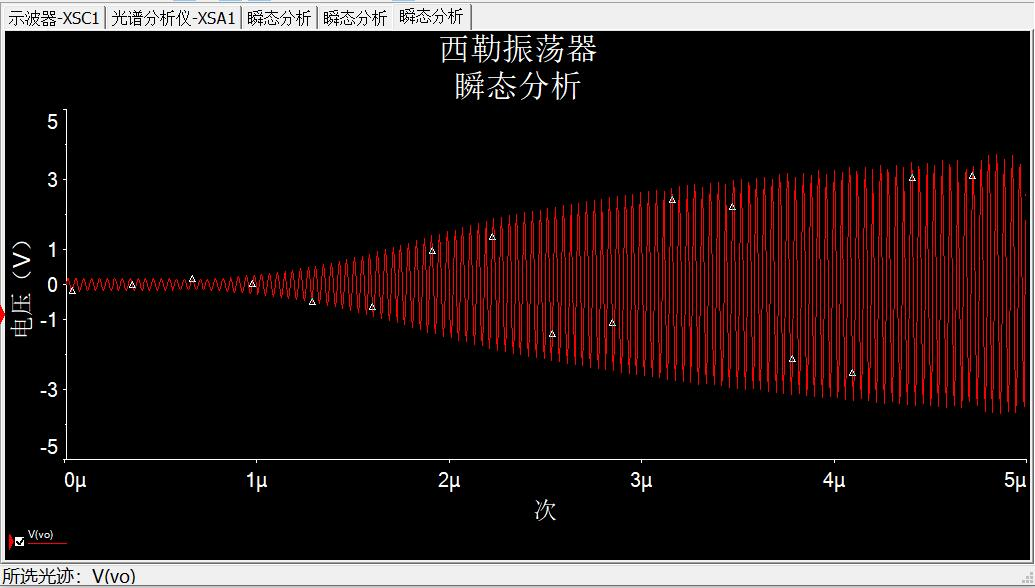
\includegraphics[width=6cm]{fig/pic5-18.jpg}
%\caption{fig1}
}
\quad
\subfigure[$C_2$ = $200pF$.]{
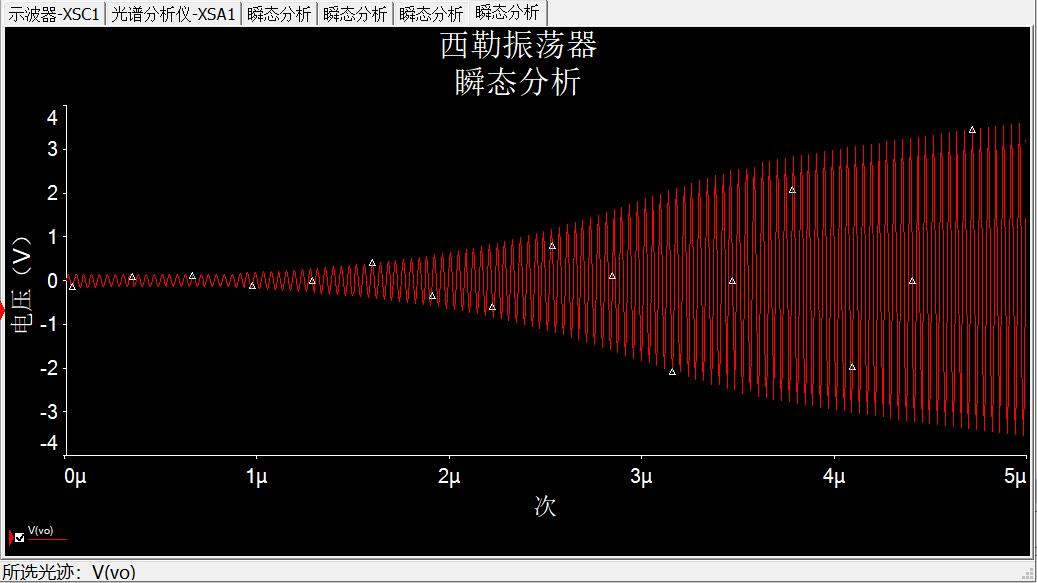
\includegraphics[width=3.9cm]{fig/pic5-19.jpg}
%\caption{fig1}
}
\quad
\subfigure[$C_2$ = $50pF$.]{
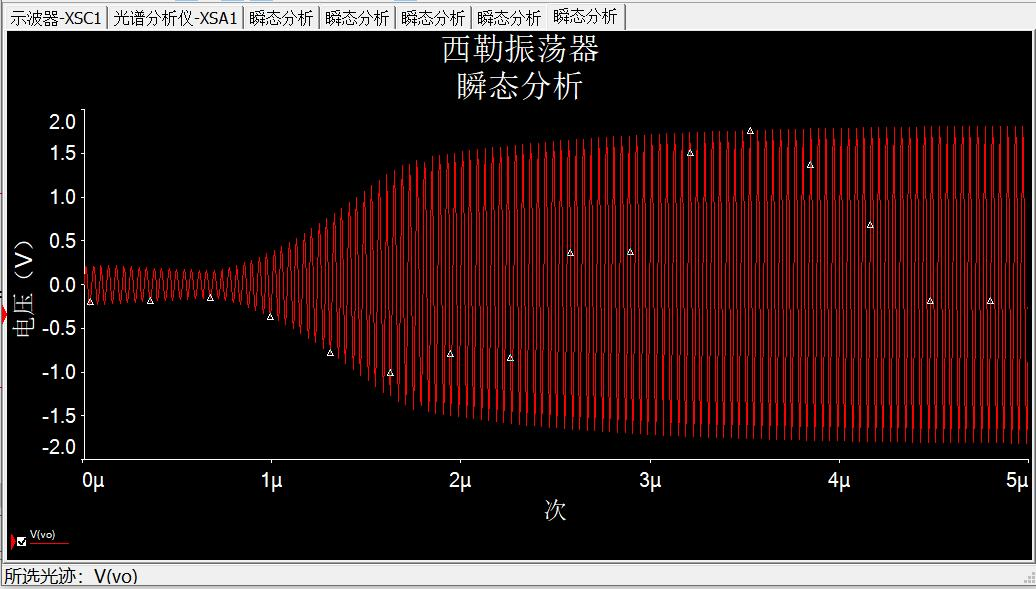
\includegraphics[width=3.9cm]{fig/pic5-20.jpg}
}
\caption{Results of changing $C_2$ in Siller Oscillator.}
\label{fig5-18/19/20}
\end{figure}

By changing $C_2$ to adjust the feedback coefficient. In the original circuit, $C_2$ = $100pF$. For comparison, increase $C2$ = $200pF$ and reduce $C2$ = $50pF$ respectively, the simulation results can be obtained in the Fig.\ref{fig5-18/19/20}-b/c. As shown in the Fig.\ref{fig5-18/19/20} -b, increasing $C_2$ makes the feedback coefficient decrease, the starting time becomes longer, and the peak-to-peak value of the output voltage increases after stabilization; while if we decrease $C_2$, the feedback coefficient increases, the starting time shortens, and the peak-to-peak value of the output voltage decreases after stabilization.

\begin{figure}[!h]
\centering
\subfigure[$C_4$ = $8pF$.]{
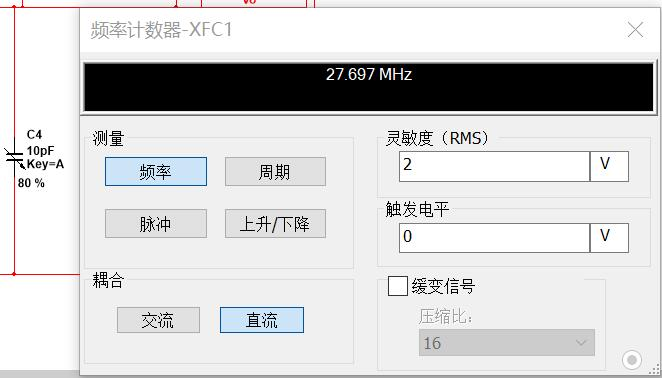
\includegraphics[width=3cm]{fig/pic5-21.jpg}
%\caption{fig1}
}
\quad
\subfigure[$C_4$ = $2pF$.]{
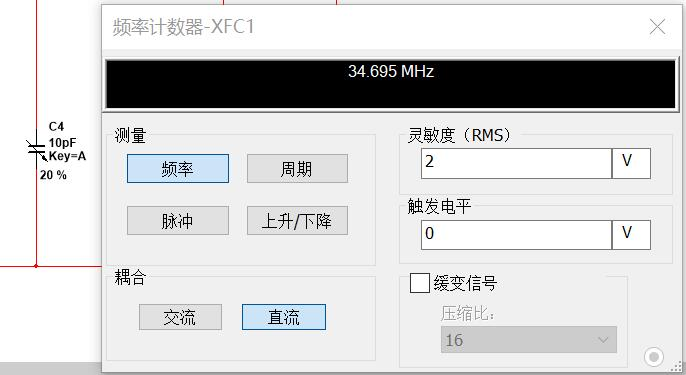
\includegraphics[width=3cm]{fig/pic5-22.jpg}
}
\caption{Results of changing $C_4$ in Siller Oscillator.}
\label{fig5-21/22}
\end{figure}

Furthermore, by changing C4 can change the oscillation frequency. In the original circuit, $C_4$ = $10pF$. By changing $C_4$ to $8pF$, $2pF$ respectively, the simulation results are shown in the Fig.\ref{fig5-21/22}. The oscillation frequency goes to $27.70MHz$ when $C_4$ = $8pF$, and the frequency goes up to $34.70MHz$ when $C_4$ = $2pF$. It can be found that as $C_4$ decreases, the oscillation frequency increases, and the time domain analysis also shows that reducing the capacitance C4 has basically no effect on the feedback coefficient.

\subsection{The three-point oscillator}
The three-point oscillator includes the capacitive and inductive type of three-point oscillator, and the schematic diagram is shown in Fig.\ref{fig5-23}. In the course of study, Hartley oscillator, Clapp oscillator can be converted into three-point oscillator using high-frequency equivalent model analysis. 

\begin{figure}[!h]
\centerline{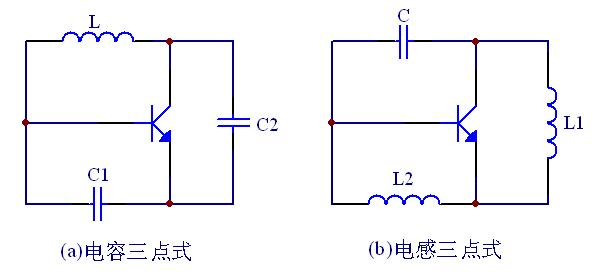
\includegraphics[scale=0.35]{fig/pic5-23.jpg}}
\caption{Three-point oscillator.}
\label{fig5-23}
\end{figure}

Since the capacitive and inductive three-point oscillators are much similar, I only simulate the inductive three-point oscillator here. The Multisim simulation circuit diagram and results are shown in Fig.\ref{fig5-24}. The oscillation frequency of the designed circuit can be derived from the frequency counter is about $955.7kHz$. 

\begin{figure}[!h]
\centerline{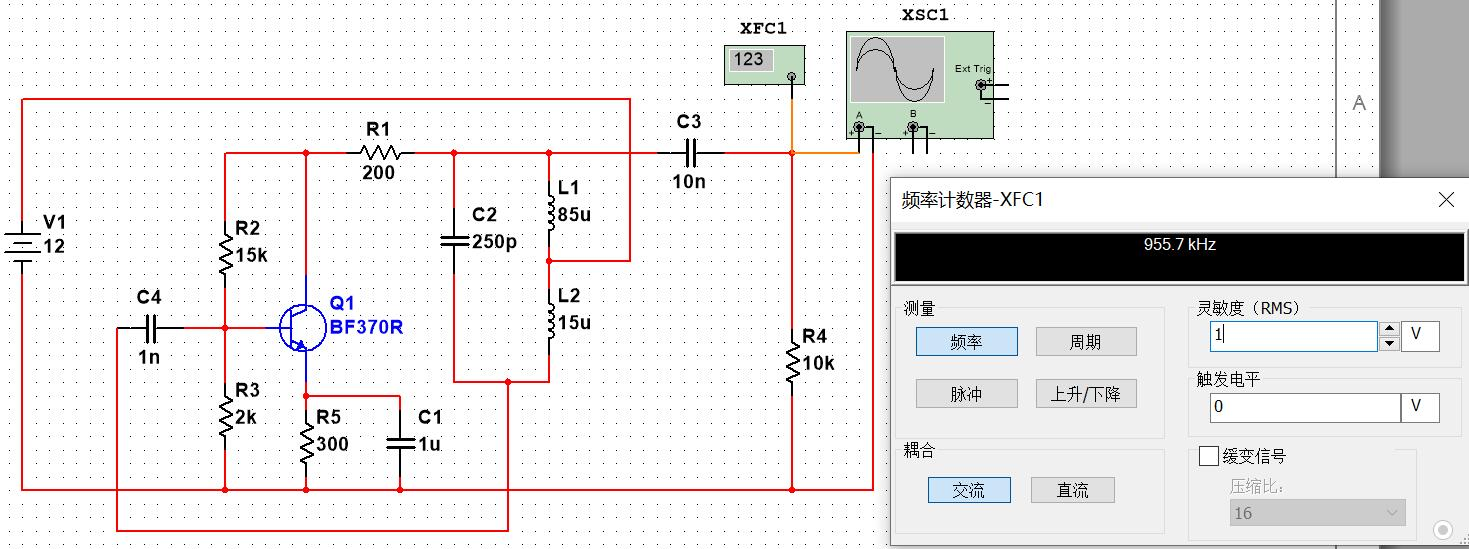
\includegraphics[scale=0.2]{fig/pic5-24.jpg}}
\caption{Simulation results of inductive three-point oscillator.}
\label{fig5-24}
\end{figure}

\section{Conclusion}\label{sec6}
This paper is based on the conference template of IEEE. It provides a brief introduction to oscillators, mainly including an introduction of the basic concepts, composition, and principles of oscillators. Besides,it includes a literature review of the important properties of oscillators, different types of oscillators. In addition, simulation experiments on several oscillators were completed using Multisim software. These works can provide fundamental help for the future both in oscillator related fields and in other communication fields.

\section*{Acknowledgment}
I am very grateful to Mrs.Gan and all the teaching assistants for your careful guidance and uncompromising assistance during this semester. I have learned a lot of basic concepts and knowledge about communication systems such as RF transceiver in this course of electronic circuits, and I have gained a lot. I also hope to apply the knowledge I learned in this course to my future studies in communications, computers, and other adjacent fields. Finally, thanks again to the teacher and all the teaching assistants!


\begin{thebibliography}{00}
\bibitem{b3} B. Razavi, "A study of phase noise in CMOS oscillators," in IEEE Journal of Solid-State Circuits, vol. 31, no. 3, pp. 331-343, March 1996, doi: 10.1109/4.494195.
\bibitem{b5} B. Razavi, "A study of injection pulling and locking in oscillators," Proceedings of the IEEE 2003 Custom Integrated Circuits Conference, 2003., 2003, pp. 305-312, doi: 10.1109/CICC.2003.1249409. 
\bibitem{b2}B. Razavi, "Mutual Injection Pulling Between Oscillators," IEEE Custom Integrated Circuits Conference 2006, 2006, pp. 675-678, doi: 10.1109/CICC.2006.320878.
\bibitem{b1} Samori C , Lacaita A L . Spectrum folding and phase noise in LC tuned oscillators[J]. IEEE Transactions on Circuits and Systems. II, 1998, 45(7):P.781-790.
\bibitem{b4} Hye-Ryoung Kim, Choong-Yul Cha, Seung-Min Oh, Moon-Su Yang and Sang-Gug Lee, "A very low-power quadrature VCO with back-gate coupling," in IEEE Journal of Solid-State Circuits, vol. 39, no. 6, pp. 952-955, June 2004, doi: 10.1109/JSSC.2004.827798.
\bibitem{b6} J. Craninckx and M. Steyaert, "Low-noise voltage-controlled oscillators using enhanced LC-tanks," in IEEE Transactions on Circuits and Systems II: Analog and Digital Signal Processing, vol. 42, no. 12, pp. 794-804, Dec. 1995, doi: 10.1109/82.476177.
\bibitem{b7} T. S. Rathore, "Synthesis and classification of LC oscillators," 2017 2nd International Conference on Communication Systems, Computing and IT Applications (CSCITA), 2017, pp. 28-32, doi: 10.1109/CSCITA.2017.8066570.
\bibitem{b8} A. Mazzanti, F. Svelto and P. Andreani, "On the amplitude and phase errors of quadrature LC-tank CMOS oscillators," in IEEE Journal of Solid-State Circuits, vol. 41, no. 6, pp. 1305-1313, June 2006, doi: 10.1109/JSSC.2006.874333.
\bibitem{b9} A. Mazzanti and P. Andreani, "A Time-Variant Analysis of Fundamental $1/f^{3}$ Phase Noise in CMOS Parallel $LC$ -Tank Quadrature Oscillators," in IEEE Transactions on Circuits and Systems I: Regular Papers, vol. 56, no. 10, pp. 2173-2180, Oct. 2009, doi: 10.1109/TCSI.2009.2015214.
\bibitem{b10} P. Andreani, A. Bonfanti, L. Romano and C. Samori, "Analysis and design of a 1.8-GHz CMOS LC quadrature VCO," in IEEE Journal of Solid-State Circuits, vol. 37, no. 12, pp. 1737-1747, Dec. 2002, doi: 10.1109/JSSC.2002.804352.
\bibitem{b11} C. Zhou, X. Zhang, F. Wang and F. Zhang, "Investigation of Non-Sinusoidal Oscillator Driven by Double Servomotors for Continuous Casting Mold," in IEEE Access, vol. 8, pp. 1235-1239, 2020, doi: 10.1109/ACCESS.2019.2958057.


\end{thebibliography}
\vspace{12pt}

\end{document}
